\newpage
\section{Problem H 从蒙德到璃月}
{ \limitfont{}
Input file: standard input \par
Output file: standard output \par
Time limit: 1000ms \par
Memory limit: 512MB \par
}
\subsection*{题目描述}

{\kaishu “向着星辰与深渊!欢迎来到冒险家协会。”}

蒙德冒险家协会的凯瑟琳让东走夕赶去璃月参加请仙典仪。可是蒙德和璃月之间的每一段道路都充满了怪物,消灭这些怪物东走夕会损失一定的生命值。由于芭芭拉小姐不愿意离开蒙德,东走夕没有恢复生命值的手段。但派蒙告诉东走夕,某些城镇中建有七天神像,东走夕可以在那里恢复满生命值。

应急食品派蒙告诉了东走夕城镇的分布,包括所有城镇之间的距离和建有七天神像城镇的位置。由于派蒙记性不好,派蒙给了每个城市一个独立的编号,这个编号从 $1$ 到 $n$,其中点 $1$ 表示出发点蒙德,$n$ 表示终点璃月。

而东走夕对自己的能力非常清楚,他明白自己在满生命值的情况下最多走 $s$ 的距离(如果东走夕在进入有七天神像的城市时刚好耗尽生命值则不会倒下)。

由于请仙典仪就要到了,东走夕希望知道在满生命值的情况下,安全的从蒙德出发到璃月的最短路程是多少。
\subsection*{输入描述}

第一行四个整数 $n,m,k,s$。

$n$ 表示城镇数量,$m(1 \leq m \leq n(n-1)/2 )$ 表示城镇之间的道路数量,$k$ 表示拥有七天神像的城镇的数量,$s$ 表示东走夕在不补充生命值情况下最多行走的距离。

第二行 $k$ 个整数,其值介于 $2$ 和 $n-1$ 之间,表示拥有七天神像的城镇。

接下来 $m$ 行每行三个整数 $a_i,b_i,w_i$,表示城镇 $a_i$ 到城市 $b_i$ 之间需要走过 $w_i$ 的路程。其中 $1 \leq a_i,b_i \leq n$。保证两个城镇之间最多只有一条路直接相连。

\subsection*{输出描述}

一个整数,输出从蒙德出发到璃月的最短路程 $Dis$,保证 $Dis < 2^{31}$。

如果无法安全到达,输出 \lstinline|"Maybe I wasn't meant for the world..."|(不包括引号。翻译:世界...拒绝了我)。

\subsection*{测试样例}

\begin{table}[H]
\begin{tabularx}{\textwidth}{|X|X|}
    \hline
    \textbf{Standard Input} & \textbf{Standard Output} \\ 
    \hline
    \tablecell{
        6 7 2 7 \\
        2 5 \\
        1 2 1 \\
        1 3 2 \\
        2 3 3 \\
        3 4 4 \\
        3 5 5 \\ 
        4 6 6 \\
        5 6 7 \\
    } & \tablecell{
        14 \\ \\ \\ \\ \\ \\ \\ \\ \\
    } \\ 
    \hline
    \tablecell{
        6 7 2 6 \\
        2 5 \\
        1 2 1 \\
        1 3 2 \\
        2 3 3 \\
        3 4 4 \\
        3 5 5 \\
        4 6 6 \\
        5 6 7 \\     
    } & \tablecell{
        Maybe I wasn't meant for the world... 
        \\ \\ \\ \\ \\ \\ \\ \\ \\
    } \\
    \hline
\end{tabularx}
\end{table}

\subsection*{数据规模}

对于$50 \%$的样例:$2 \leq n \leq 10,1\leq s < 10000,1 \leq w_i < 1000$。

对于$100 \%$的样例:$2 \leq n \leq 500,1\leq s < 2^{31},1 \leq w_i < 2^{21}$。

\subsection*{样例解释}

对于样例 $1$,东走夕走到点3时最多还可以在走 $5$ 米,虽然 $3 \rightarrow 4 \rightarrow 6$ 在路程上更近,但东走夕会因为生命值耗尽倒下,所以只能选择下方 $3 \rightarrow 5 \rightarrow 6$ 的路径。

\begin{figure}[H]
    \centering
    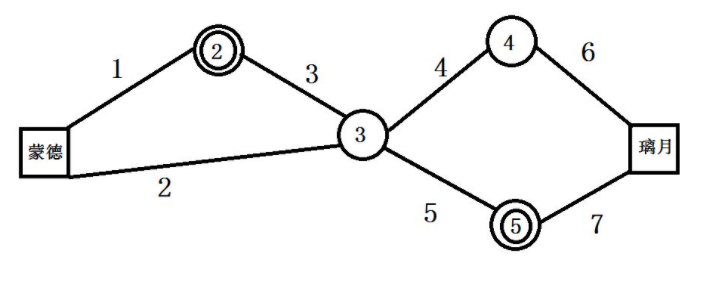
\includegraphics[scale=0.6]{./src/Problem-H-1.png}
\end{figure}

对于样例2,东走夕无论怎么走都会倒下,所以输出 \lstinline|"Maybe I wasn't meant for the world..."|。